\documentclass{article}   

\usepackage{geometry}
\usepackage{qtree}
\usepackage[square,numbers]{natbib}
% \usepackage{cite}  
\geometry{a4paper}

\usepackage[]{algorithm2e}
\usepackage{amsthm}
\newtheorem{theorem}{Theorem}[section]
\newtheorem{corollary}{Corollary}[theorem]
\newtheorem{lemma}[theorem]{Lemma}

\usepackage[utf8]{inputenc}
\usepackage[T1]{fontenc}    % use 8-bit T1 fonts
\usepackage{lmodern}
\usepackage{hyperref}       % hyperlinks
\usepackage{lipsum}

\usepackage{color, colortbl}

\definecolor{Gray}{gray}{0.9}

\usepackage[protrusion=true,expansion=true]{microtype}

\usepackage{amssymb}
\usepackage{amsfonts}
\usepackage{eqnarray,amsmath}
\usepackage[table]{xcolor}

\usepackage{listings}
\usepackage{graphicx}
\usepackage{dirtytalk}

\usepackage{rotating}
\usepackage{caption}

%% if you use PostScript figures in your article
%% use the graphics package for simple commands
\usepackage{graphics}


%% or use the graphicx package for more complicated commands
\usepackage{graphicx}
\usepackage[table]{xcolor}

\usepackage{indentfirst}
\usepackage[utf8]{inputenc}
 \usepackage{subcaption}
\usepackage{xcolor}
 
\usepackage{xspace,color}
\usepackage{url}



\lstset{commentstyle=\color{red},keywordstyle=\color{black},
showstringspaces=false}
\lstnewenvironment{rc}[1][]{\lstset{language=R}}{}
\newcommand{\ri}[1]{\lstinline{#1}}  %% Short for 'R inline'

\lstset{language=R}             % Set R to default language


%https://tex.stackexchange.com/questions/96825/nicely-formatted-where-statement-for-maths
 \newenvironment{where}{\noindent{}where\begin{itemize}}{\end{itemize}}
 \renewcommand*\descriptionlabel[1]{\hspace\leftmargin$#1$}
 
\lstset{escapeinside={<@}{@>}}
% please place your own definitions here and don't use \def but
% \newcommand{}{}
%
% Insert the name of "your journal" with
% \journalname{myjournal}
%
\begin{document}

\title{%
  Practice 5: Pseudo Random Numbers} %\\~\\
  %\Large }
\author{Mayra Cristina Berrones Reyes 6291}

\maketitle

\section{Introduction}

A pseudo random number is the term used for the computer generated random numbers. The prefix \say{pseudo} is used be differentiate this type of number to a truly random number that is generated by a random physical process such as radioactive decay \cite{w-pseudo}. \\

A pseudo random number generator (PRNG) is refereeing to an algorithm that uses mathematical formulas to create sequences that approximate as much as posible random numbers. This type of numbers are very important in the area of computational science, because more often than not, we find the need to use randomness in a computer program to be able to perform experiments. It is quite difficult however, to get a computer to do something by chance, because a computer follows instructions in a way that can be predicted one way or another \cite{geeks1}. \\

Truly random numbers are not possible to generate from a deterministic method, so we use PRNG techniques to develop random numbers using a computer. A PRNG sequence is completely determined by an initial value called seed. \\

\section{Generators based on linear recurrences}\label{gen}

A great discovery in pseudo random generators was the introduction of techniques based on linear recurrences. They where used as standard in the second half of the 20th century. Their quality was known to be inadequate, but there were no better methods available. \\

A linear congruential generator (LCG) in an algorithm used to make pseudo randomized numbers with a discontinuous piecewise linear equation. This generator is defined by the recurrence relation represented in Equation \ref{eq1}:\\

\begin{equation} \label{eq1}
X_{n+1} = (aX_n + c) \mbox{\texttt{ mod }} m
\end{equation}
where:
\begin{description}
\item[\textit{m}] $0 < m - $ the \say{modulus}
\item[\textit{a}] $0 < a < m -$ the \say{multiplier} 
\item[\textit{c}] $0 \leq c < m -$ the \say{increment} 
\item[\textit{$X_0$}] $0 \leq  X_0 < m - $ the \say{seed} 
\end{description}

Given this generator, for this experimentation we are working with three different examples of LCG. First we have the standard generator of R for uniform random numbers \texttt{runif}. The other one is one generated by code shown in \ref{code1}, where the variables \texttt{a, c,} and \texttt{m} in Equation \ref{eq1} are prime numbers. The seed used is fixed to 27.\\

\begin{lstlisting}[caption = Code for uniform random numbers in R, label=code1]
> uniforme = <@\textcolor{blue}{function}@>(n, semilla) {
>    a = <@\textcolor{blue}{11551}@>
>    c = <@\textcolor{blue}{27077}@>
>    m = <@\textcolor{blue}{39709}@>
>    datos = numeric()
>    x = semilla
>    <@\textcolor{blue}{while}@> (length(datos) < n) {
+        x = (a * x + c) <@\textcolor{gray}{\%\%}@> m
+        datos = c(datos, x)
>    }
>    <@\textcolor{blue}{return}@>(datos / (m - <@\textcolor{blue}{1}@>))
>    }
\end{lstlisting}


The third generator uses the same structure as \ref{code1}, but the values of \texttt{a, c,} and \texttt{m} are taken from the experimentation in the ANSI experimentation by Saucier \cite{saucier}, \texttt{m} $= 2^{32}$, \texttt{a} $=$ 1103515245 and \texttt{c} $=$ 12345. Another main difference is the quality of the seed used. In this case we set the seed using the current system time in microseconds.\\ 

On all three we perform a uniform test with a Chi - squared. In all three the \texttt{p value} gives us a correct uniformity, as shown in Figure \ref{fig1}.\\

\begin{figure}[]
\begin{subfigure}{.33\textwidth}
  \centering
  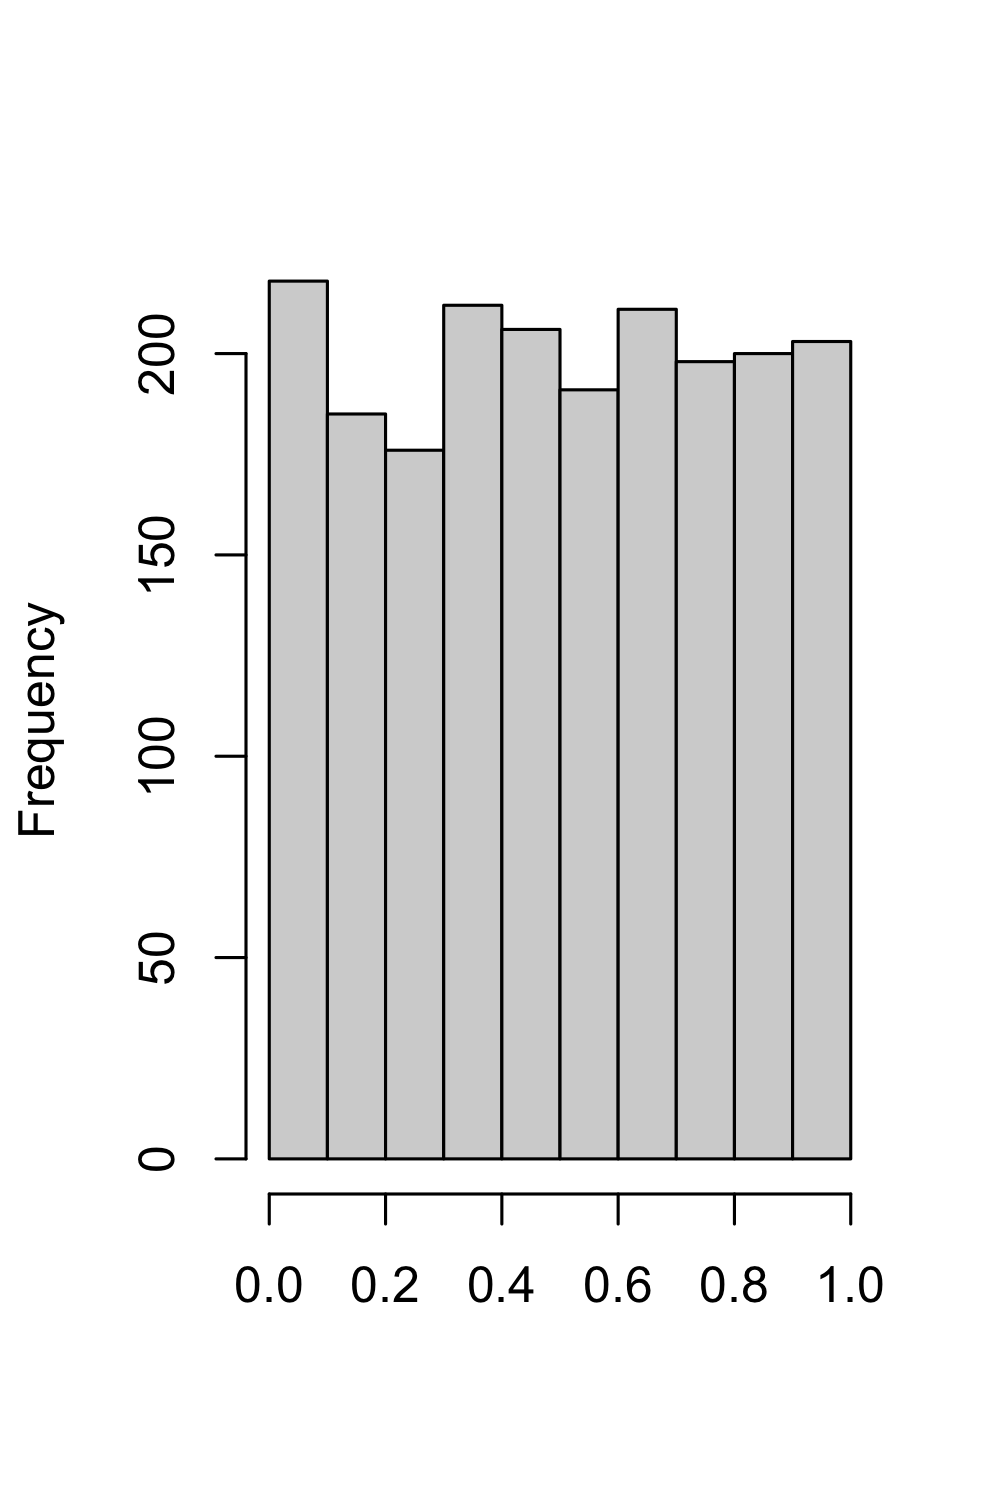
\includegraphics[width=1\linewidth]{Ej5_runif.png}  
  \caption{Histogram of \texttt{runif} (2000) }
  \label{subfig1-1}
\end{subfigure}
\begin{subfigure}{.33\textwidth}
  \centering
  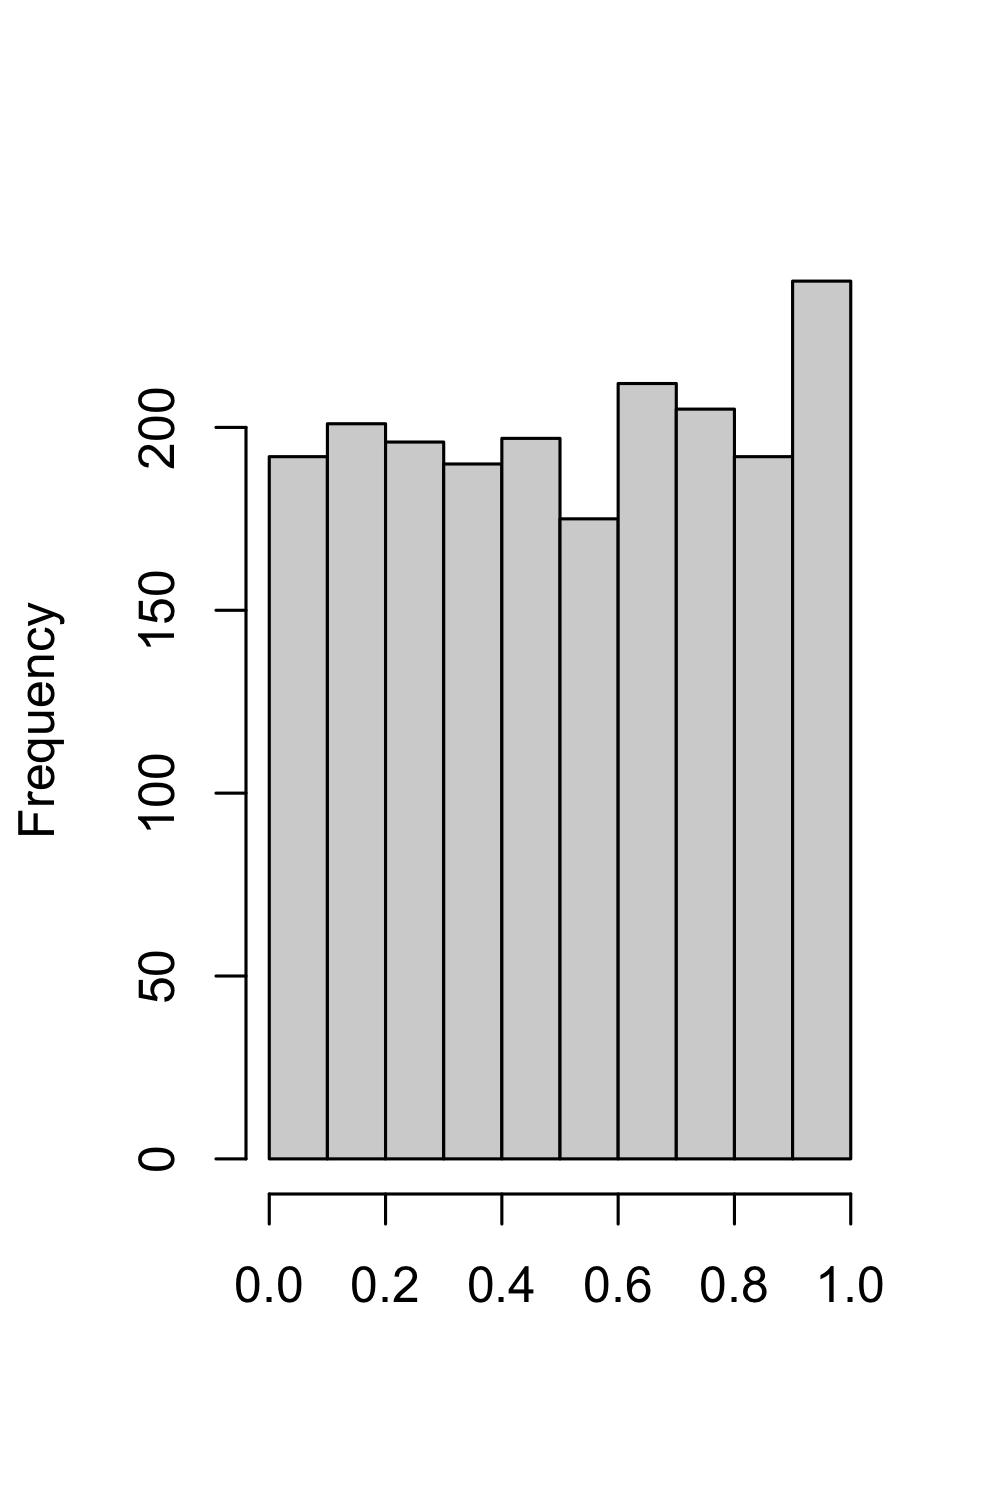
\includegraphics[width=1\linewidth]{Ej5_uniforme.png}  
  \caption{Histogram of function \texttt{uniforme}(2000, 27)}
  \label{subfig1-2}
\end{subfigure}
\begin{subfigure}{.33\textwidth}
  \centering
  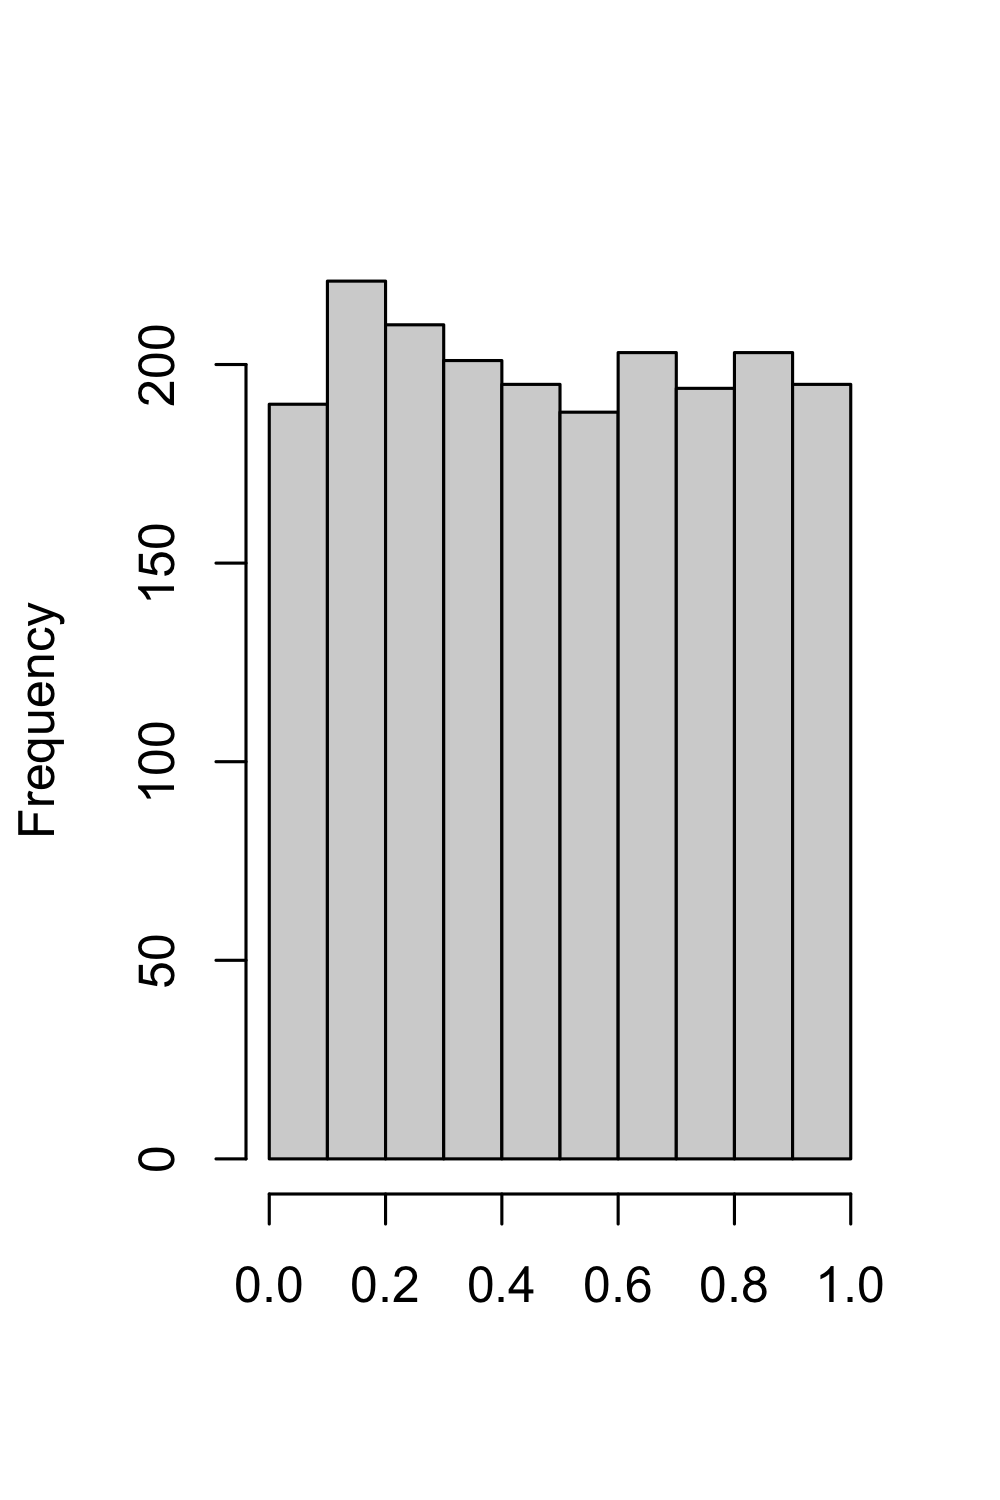
\includegraphics[width=1\linewidth]{Ej5_lcg.png}  
  \caption{Histogram of function \texttt{lcg.rand}(2000)}
  \label{subfig1-3}
\end{subfigure}
\caption{Histograms showing the behaviours of each experimentation.}
\label{fig1}
\end{figure}

\clearpage


\section{Gaussian distribution}

The Gaussian distribution, also known as normal distribution, in probability theory is a type of continuous probability distribution for a real valued random variable. The form of its probability density is shown in Equation \ref{eq2}. \\

\begin{equation} \label{eq2}
f(x) = \frac{1}{\sigma\sqrt{2 \pi}}e^{-\frac{1}{2} \left(\frac{x-\mu}{\sigma}\right)^2 }
\end{equation}
where:
\begin{description}
\item[\textit{$\mu$}] is the mean or expectation of the distribution.
\item[\textit{$\sigma$}] is the standard deviation.
\item[\textit{$\sigma^2$}] is the variance of the distribution.
\end{description}

A random variable with this Gaussian distribution is called normal deviate. \\

Using the standard Box -- Muller transform we are experimenting using the three generators of uniform random numbers mentioned in Section \ref{gen} and moving the values of $Z$. If $Z$ is a standard normal deviate then $X=Z\sigma + \mu$ will have a normal distribution \cite{muller}. \\

\begin{lstlisting}[caption = Code for Gaussian distribution in R, label=code2]
> gaussian = <@\textcolor{blue}{function}@>(mu, sigma) {
>    u = runif(<@\textcolor{blue}{2}@>);
>    z0 = sqrt(<@\textcolor{blue}{-2}@> * log(u[<@\textcolor{blue}{1}@>])) * cos(<@\textcolor{blue}{2}@> * pi * u[<@\textcolor{blue}{2}@>]);
>    z1 = sqrt(<@\textcolor{blue}{-2}@> * log(u[<@\textcolor{blue}{1}@>])) * sin(<@\textcolor{blue}{2}@> * pi * u[<@\textcolor{blue}{2}@>]);
>    datos = c(z0, z1);
>    <@\textcolor{blue}{return}@> (sigma * datos + mu);
>  }

cat(gaussian(<@\textcolor{blue}{0}@>, <@\textcolor{blue}{1}@>))
\end{lstlisting}

In Figure \ref{fig5} we see all the distributions for all the experimentations with the different parameters using the code in Listing \ref{code2}. On Figures \ref{subfig5-1}, \ref{subfig5-2} and \ref{subfig5-3} we use both parameters $Z_0$ and $Z_1$. As we can appreciate Figures \ref{subfig5-1} and \ref{subfig5-3} behave as a normal distribution. Changing the parameter used to only $Z_0$ made little difference in those two distributions, as we can see in Figures \ref{subfig5-4} and \ref{subfig5-6}, but in the case of Figure \ref{subfig5-5} it changes quite a bit. \\

In an effort to normalize whatever was happening on Figures \ref{subfig5-2} and \ref{subfig5-5} we used the two random generated numbers as separated variables \texttt{u1} and \texttt{u2} with the two $Z$ variables. In Figure \ref{subfig5-7} the parameter for \texttt{u1} is \texttt{runif}(1) and \texttt{u2} we use the function \texttt{uniforme} (1, \texttt{u1} $*$ 1000).\\

Then in Figure \ref{subfig5-8} we tried the same using now \texttt{u1} as the function \texttt{lcg.rand} (1) and \texttt{u2} \texttt{uniforme} (1, \texttt{u1} $*$ 1000). Both of this figures behave as normal distributions. Thinking that the solution to the \texttt{uniforme} function was the variables, we made a last attempt. In Figure \ref{subfig5-9} we used \texttt{u1} as the function \texttt{uniforme} (1, 27) and \texttt{u2} \texttt{uniforme} (1, \texttt{u1} $*$ 1000). This however yielded the same results as using the \texttt{uniforme} function by itself.\\

\begin{figure}[]
\begin{subfigure}{.33\textwidth}
  \centering
  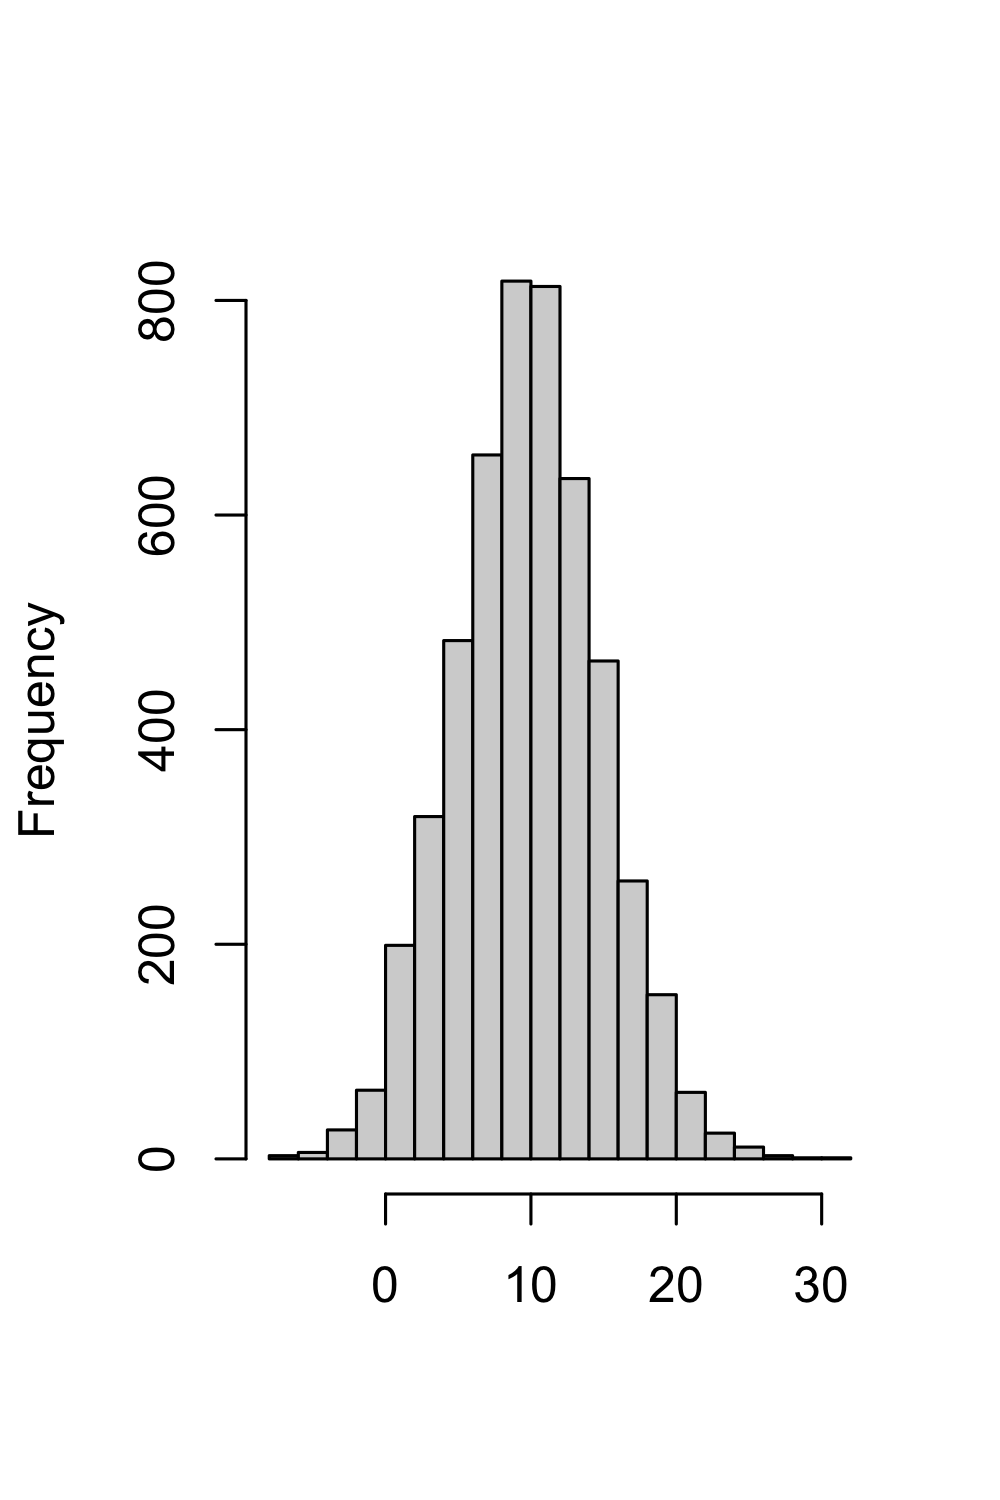
\includegraphics[width=.8\linewidth]{Ej5_h1_runif.png}  
  \caption{With $Z_0$ and $Z_1$ using \texttt{runif}}
  \label{subfig5-1}
\end{subfigure}
\begin{subfigure}{.33\textwidth}
  \centering
  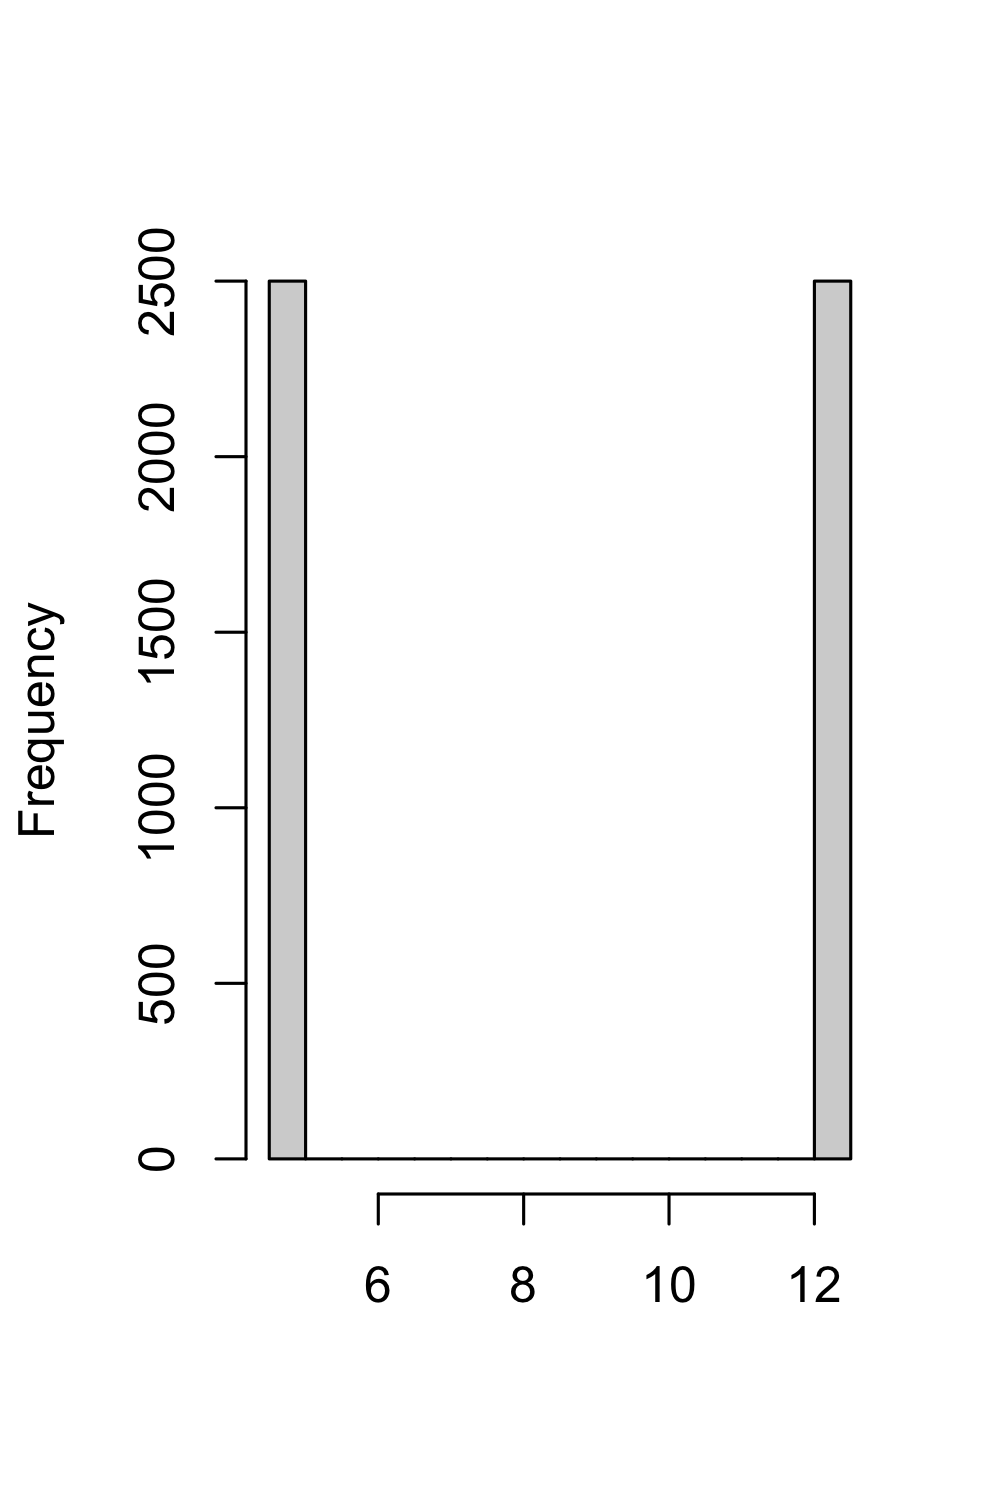
\includegraphics[width=.8\linewidth]{Ej5_h1_uniforme.png}  
  \caption{With $Z_0$ and $Z_1$ using \texttt{uniforme} function}
  \label{subfig5-2}
\end{subfigure}
\begin{subfigure}{.33\textwidth}
  \centering
  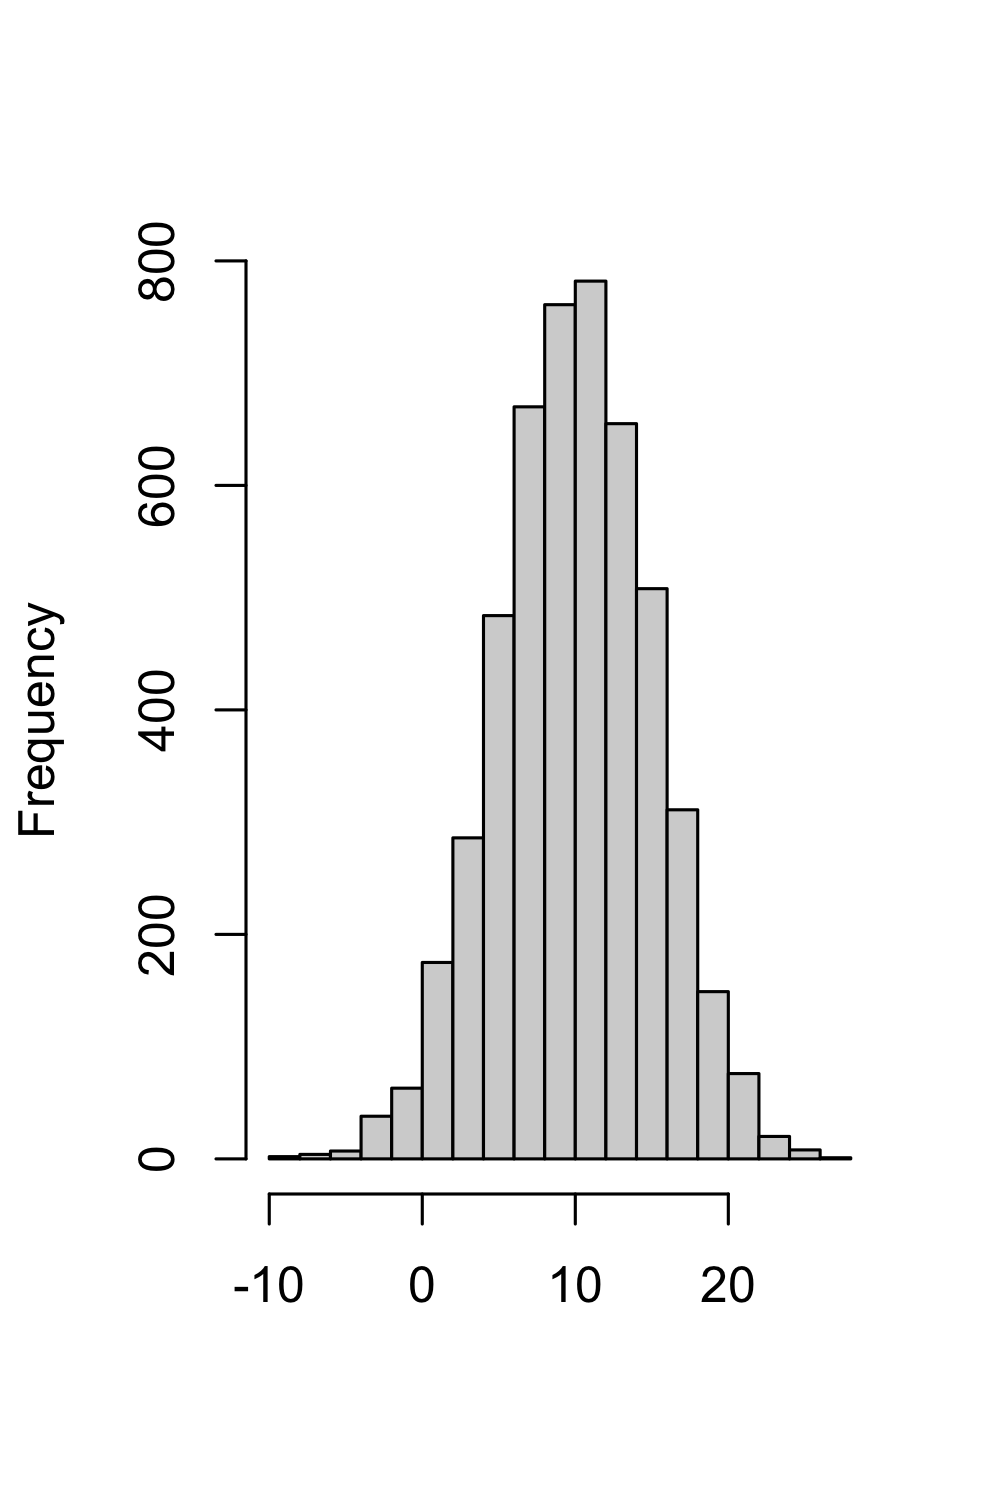
\includegraphics[width=.8\linewidth]{Ej5_h1_lcg.png}  
  \caption{ With $Z_0$ and $Z_1$ using \texttt{lcg} function}
  \label{subfig5-3}
\end{subfigure}
\newline
\begin{subfigure}{.33\textwidth}
  \centering
  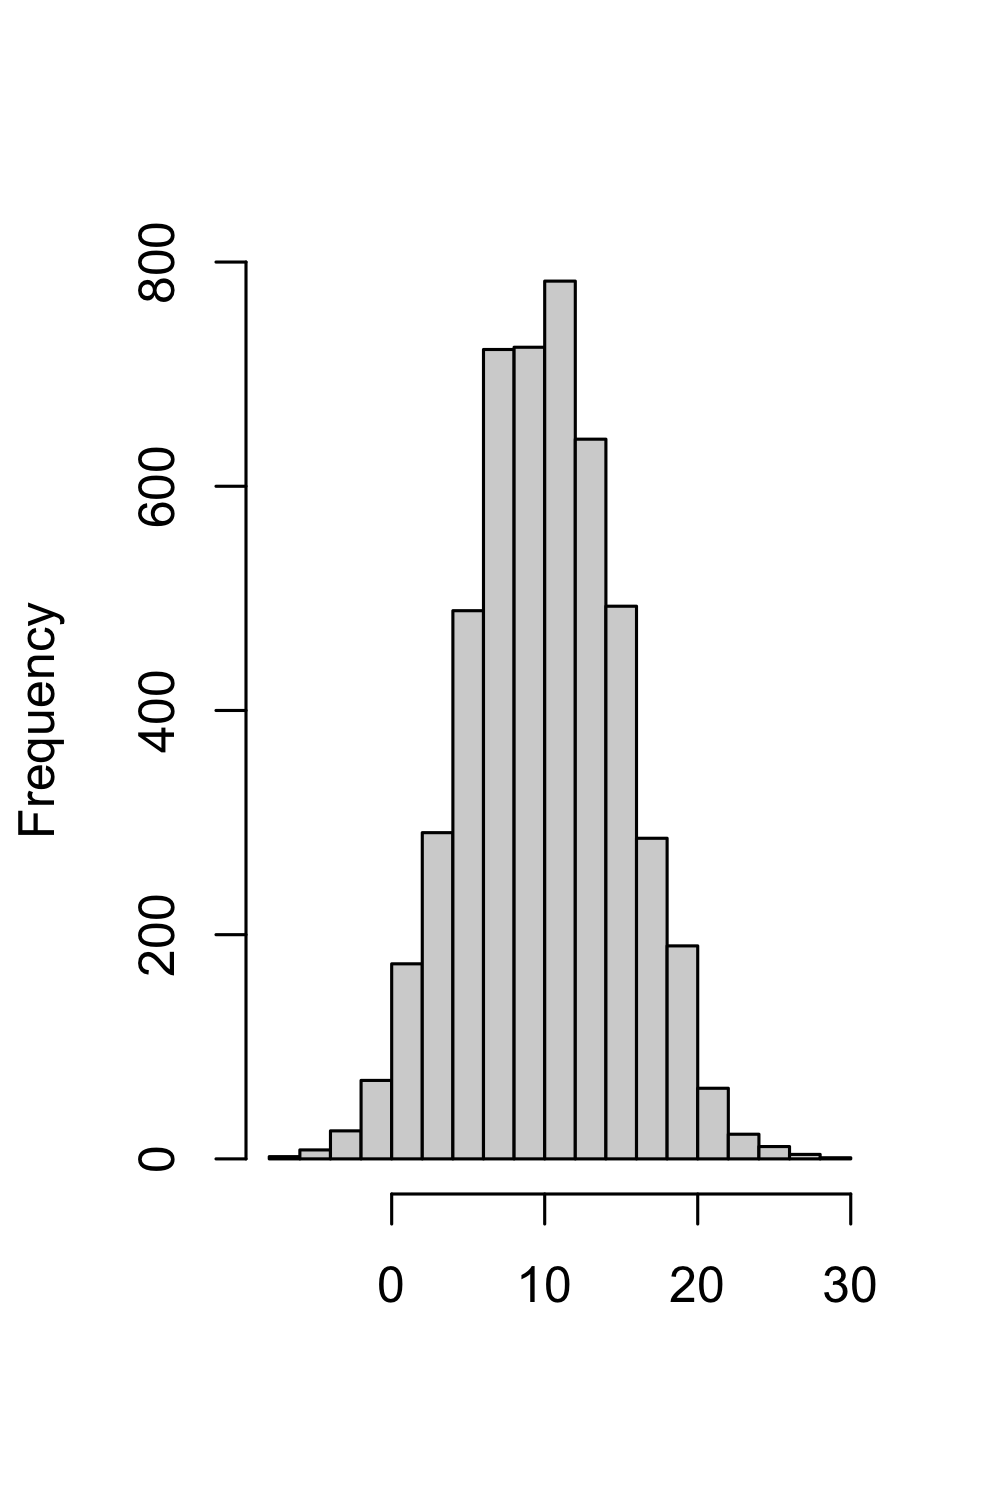
\includegraphics[width=.8\linewidth]{Ej5_z0_runif.png}  
  \caption{With $Z_0$ using \texttt{runif}}
  \label{subfig5-4}
\end{subfigure}
\begin{subfigure}{.33\textwidth}
  \centering
  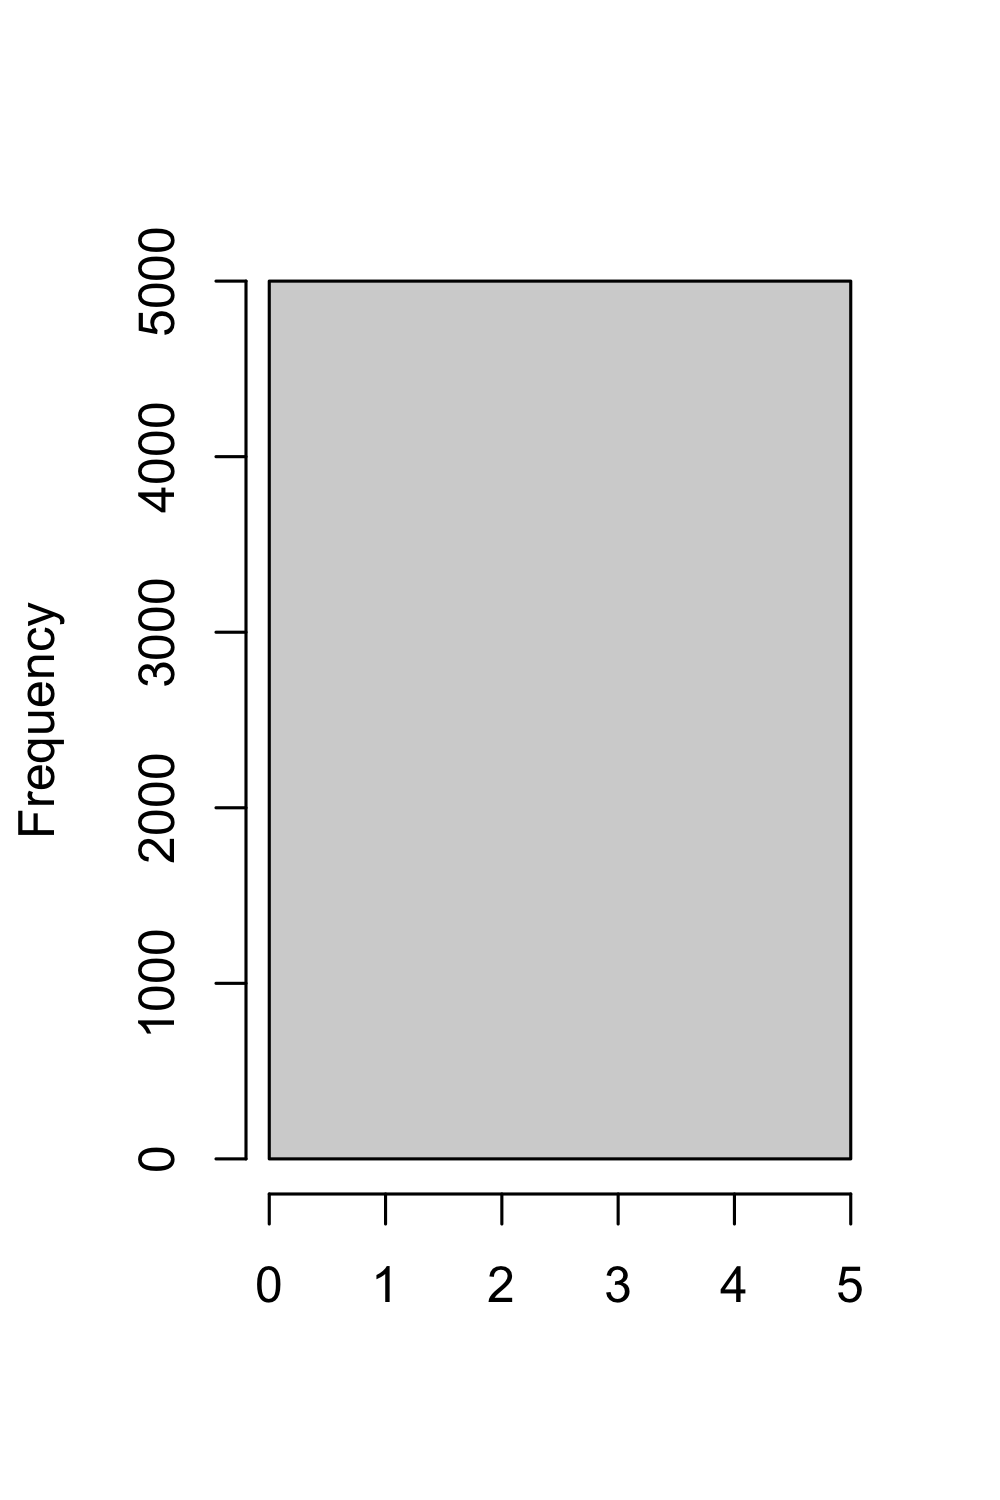
\includegraphics[width=.8\linewidth]{Ej5_z0_uniforme.png}  
  \caption{With $Z_0$ using \texttt{uniforme} function}
  \label{subfig5-5}
\end{subfigure}
\begin{subfigure}{.33\textwidth}
  \centering
  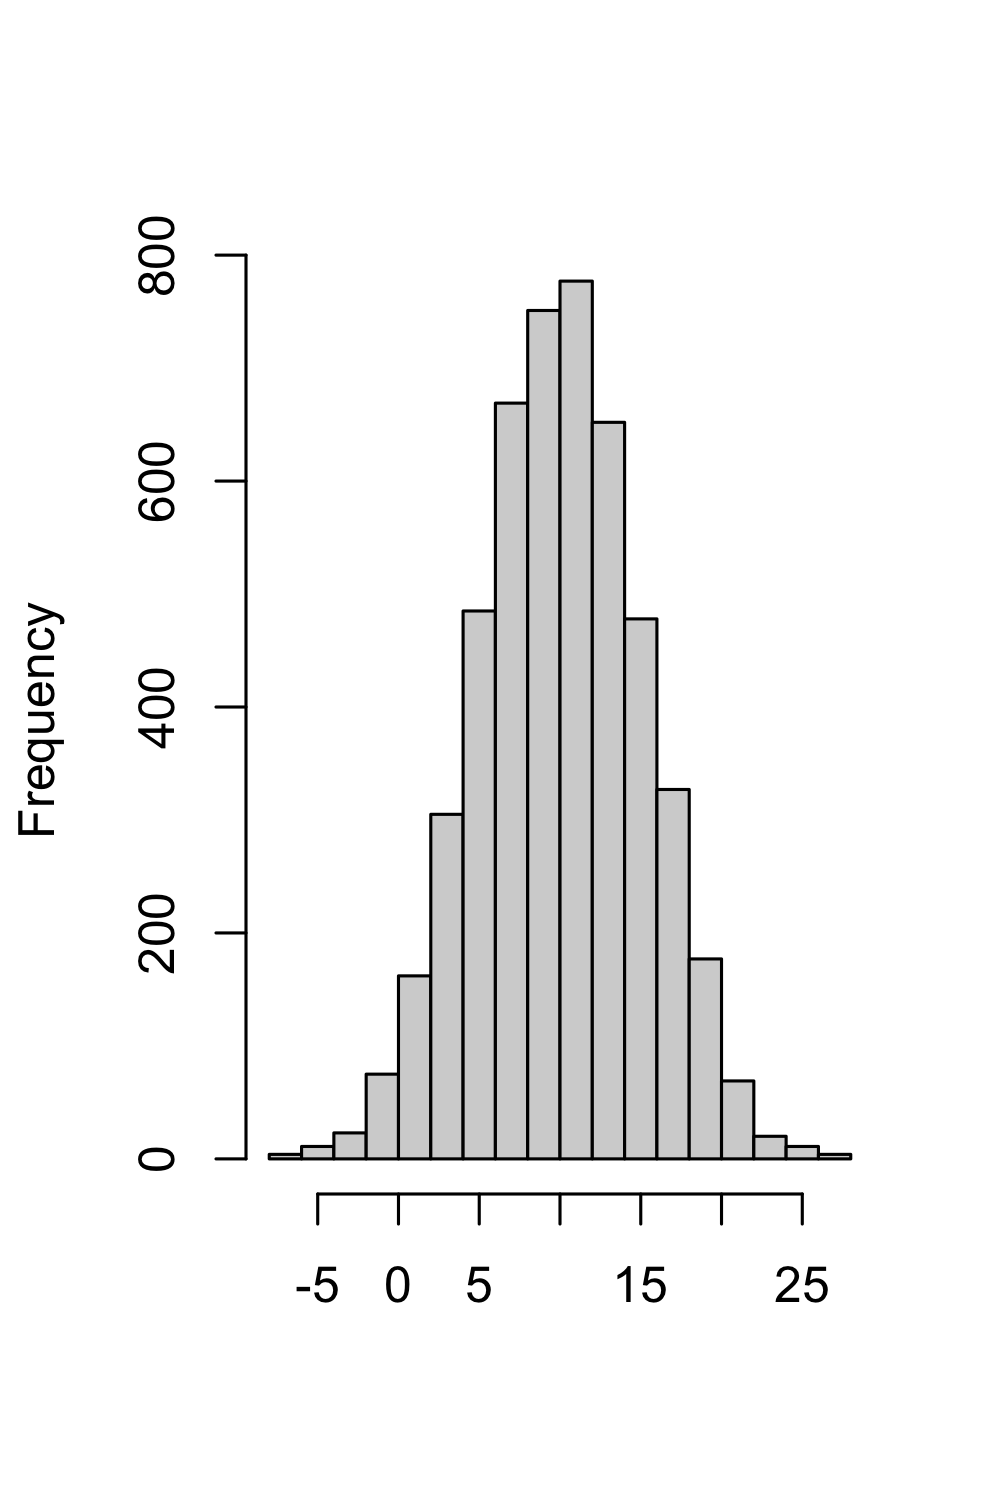
\includegraphics[width=.8\linewidth]{Ej5_z0_lcg.png}  
  \caption{With $Z_0$ using \texttt{lcg} function}
  \label{subfig5-6}
\end{subfigure}
\newline
\begin{subfigure}{.33\textwidth}
  \centering
  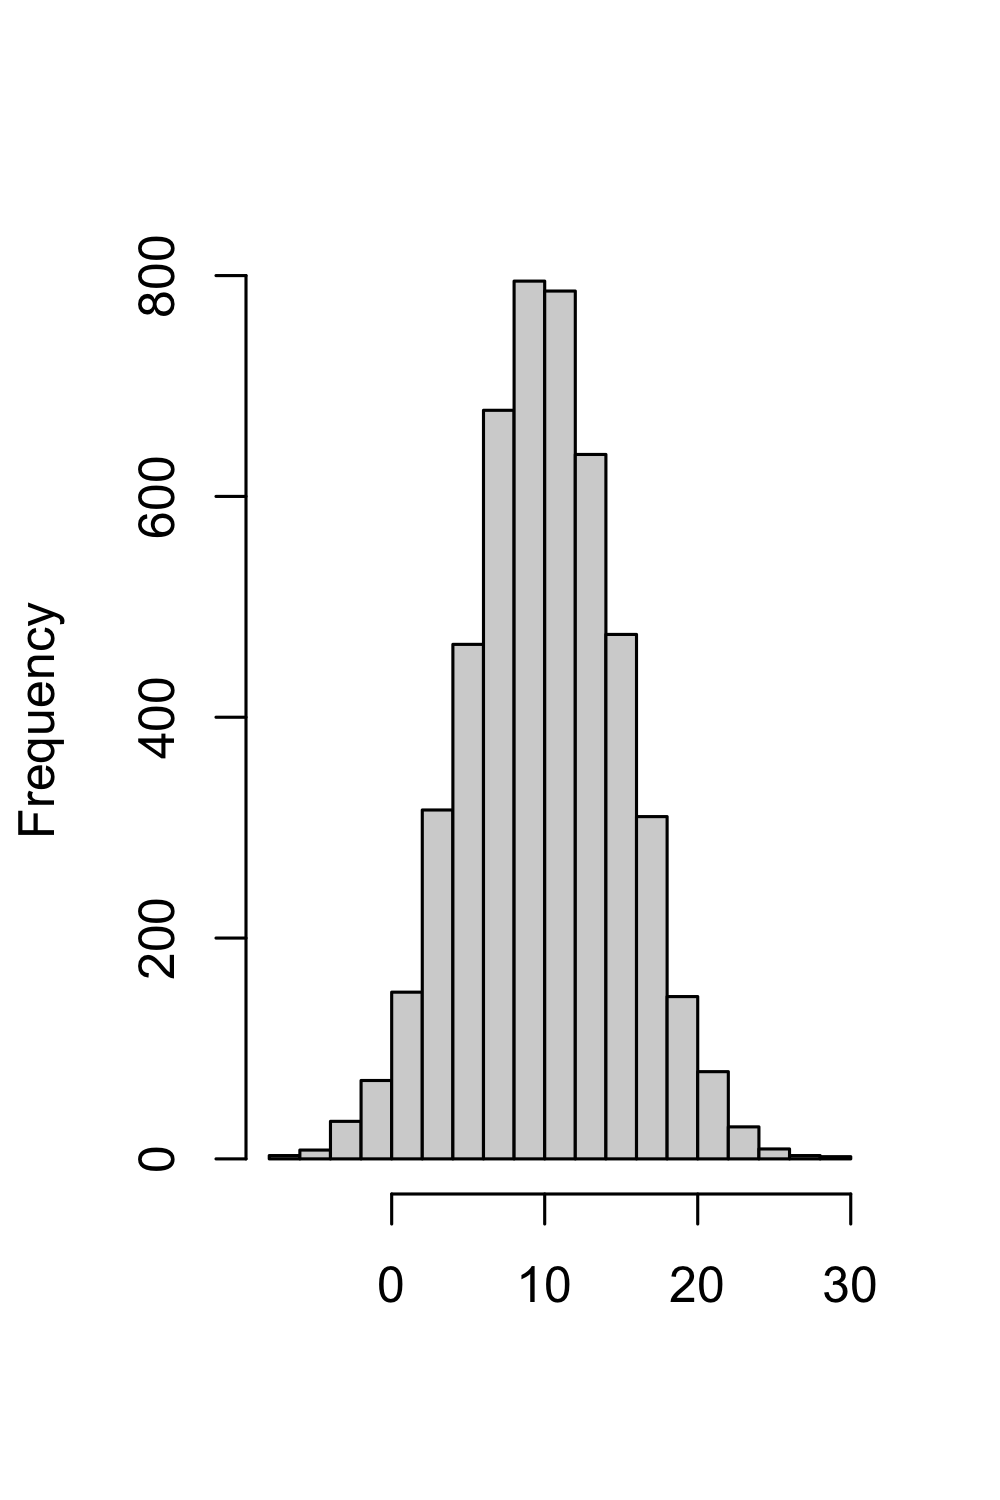
\includegraphics[width=.8\linewidth]{Ej5_run_uni.png}  
  \caption{With $Z_0$ and $Z_1$ using \texttt{runif} as u1 and \texttt{uniforme} as u2}
  \label{subfig5-7}
\end{subfigure}
\begin{subfigure}{.33\textwidth}
  \centering
  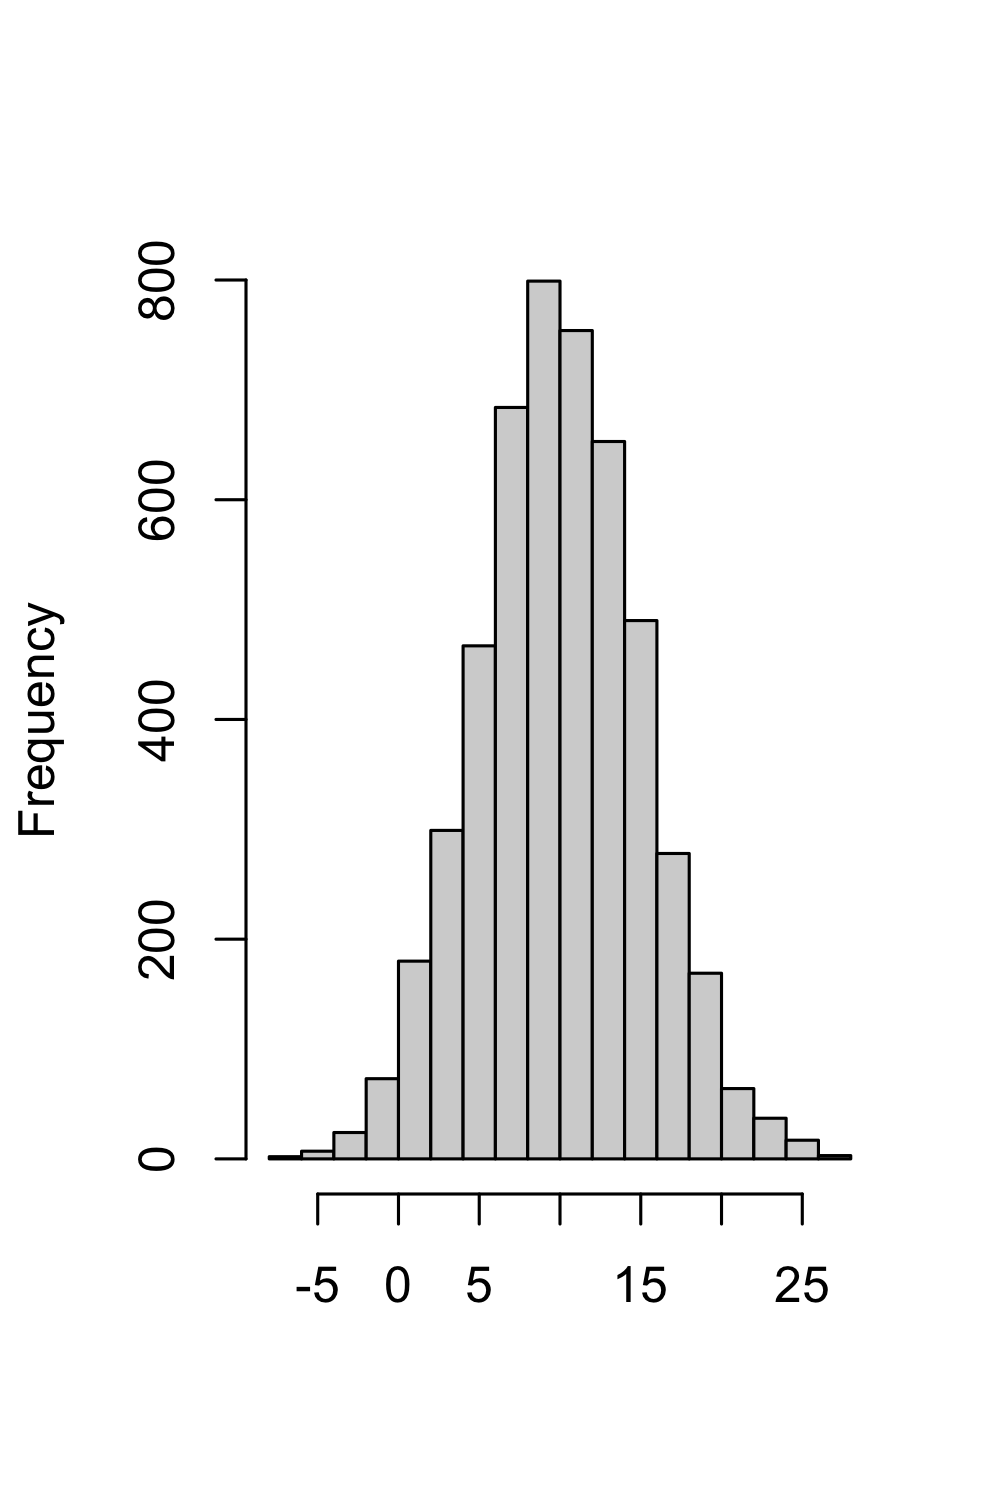
\includegraphics[width=.8\linewidth]{Ej5_uni_lcg.png}  
  \caption{With $Z_0$ and $Z_1$ using \texttt{lcg} as u1 and \texttt{uniforme} as u2}
  \label{subfig5-8}
\end{subfigure}
\begin{subfigure}{.33\textwidth}
  \centering
  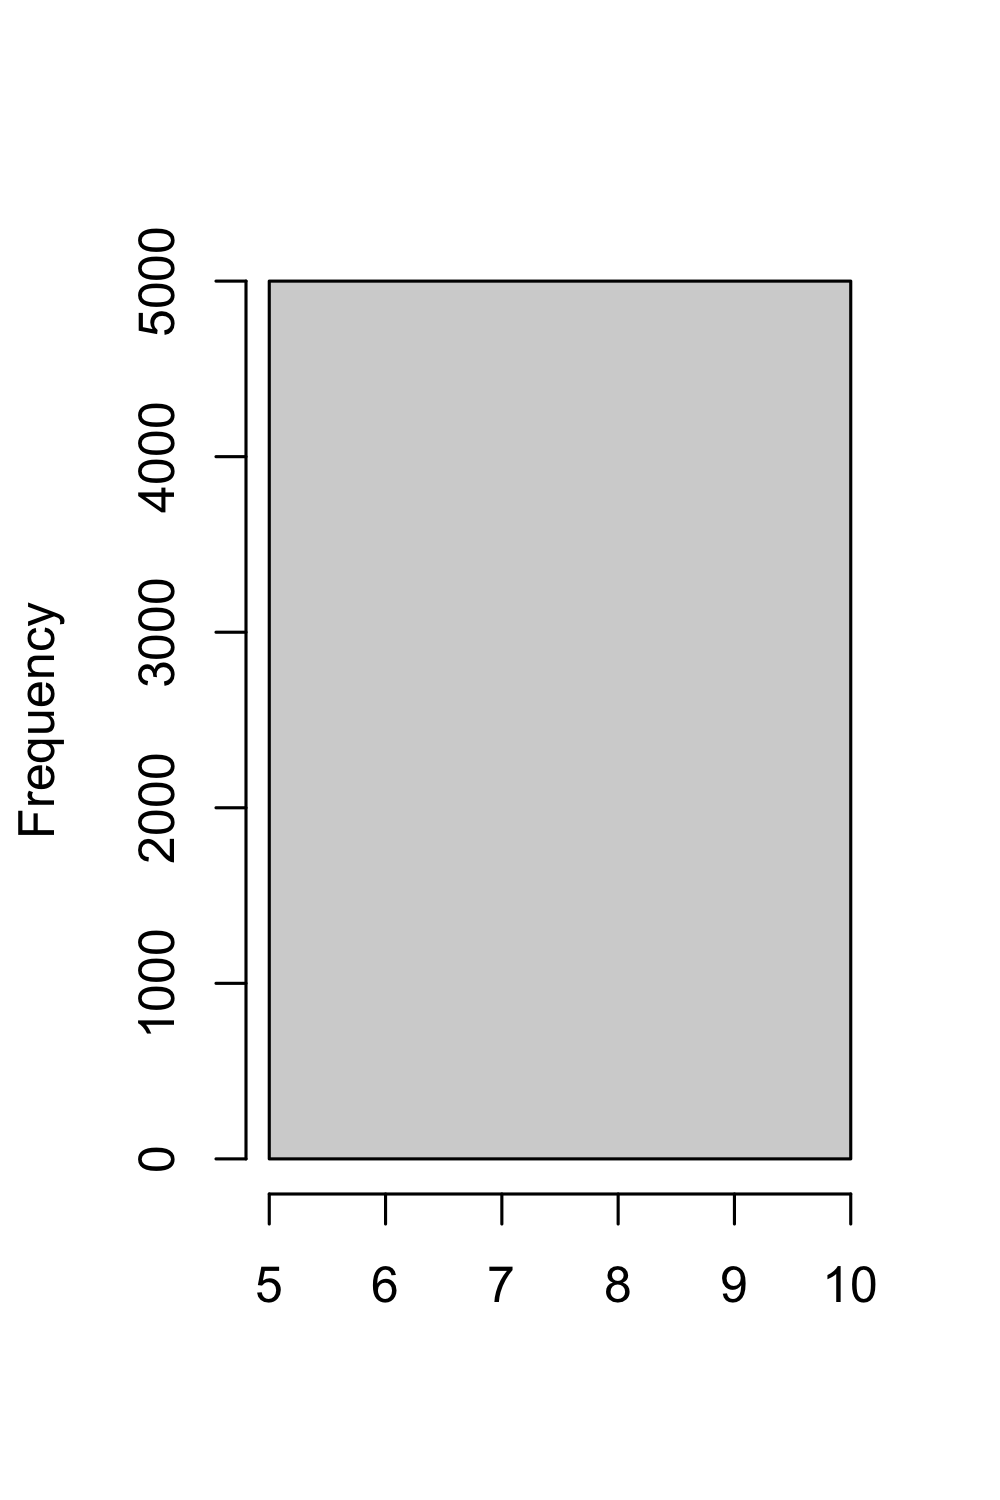
\includegraphics[width=.8\linewidth]{Ej5_uni_unif.png}  
  \caption{With $Z_0$ and $Z_1$ using \texttt{uniforme} as u1 and \texttt{uniforme} as u2}
  \label{subfig5-9}
\end{subfigure}
\caption{Histograms of all the distributions with different parameters.  }
\label{fig5}
\end{figure}

\clearpage

\section{Other experiments}

Looking for a better seed for the experimentation of the uniform distribution, we arrived to an example of a different way of seeing the randomness of each experimentation. In Figure \ref{extra} we can see in each point the behaviour of the \texttt{runif}, the \texttt{lcg} and the \texttt{uniforme} functions.\\

Same as with the distributions plot, in this figure we see an odd behaviour on the \texttt{uniforme} function.\\


\begin{figure}[]
\begin{subfigure}{.5\textwidth}
  \centering
  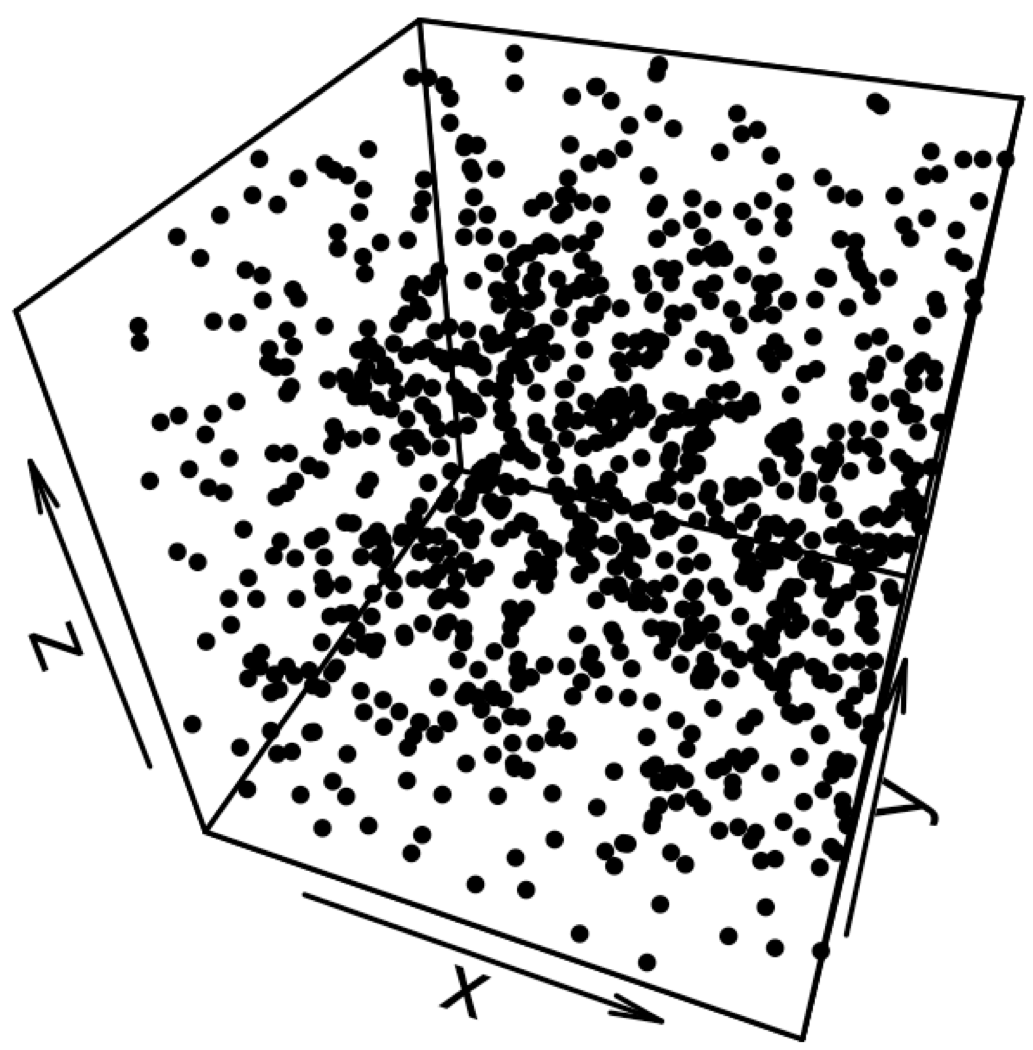
\includegraphics[width=.8\linewidth]{Ej5_scrunif.png}  
  \caption{3D of \texttt{runif} (2000) }
  \label{extra1}
\end{subfigure}
\begin{subfigure}{.5\textwidth}
  \centering
  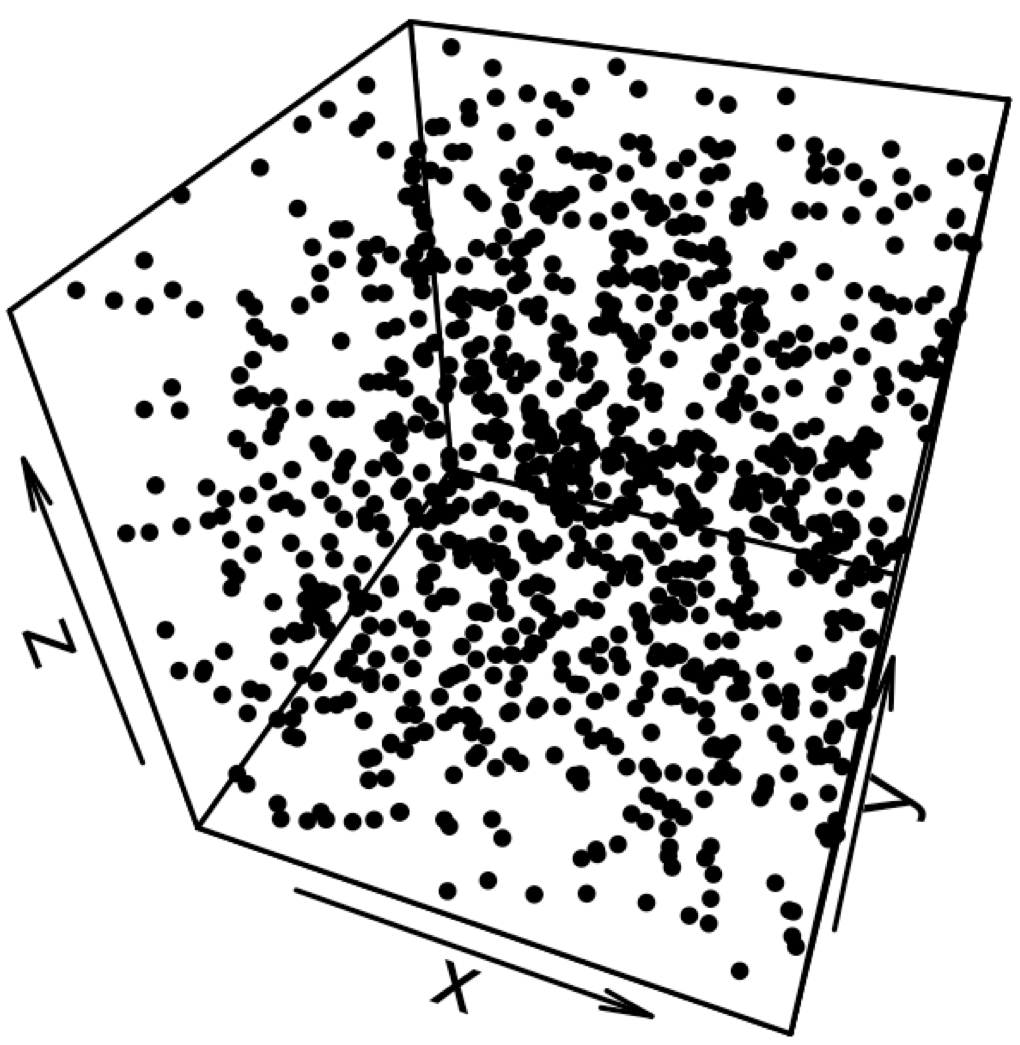
\includegraphics[width=.8\linewidth]{Ej5_sclcg.png}  
  \caption{3D of function \texttt{lcg.rand}(2000)}
  \label{extra2}
\end{subfigure}
\newline
\begin{subfigure}{.5\textwidth}
  \centering
  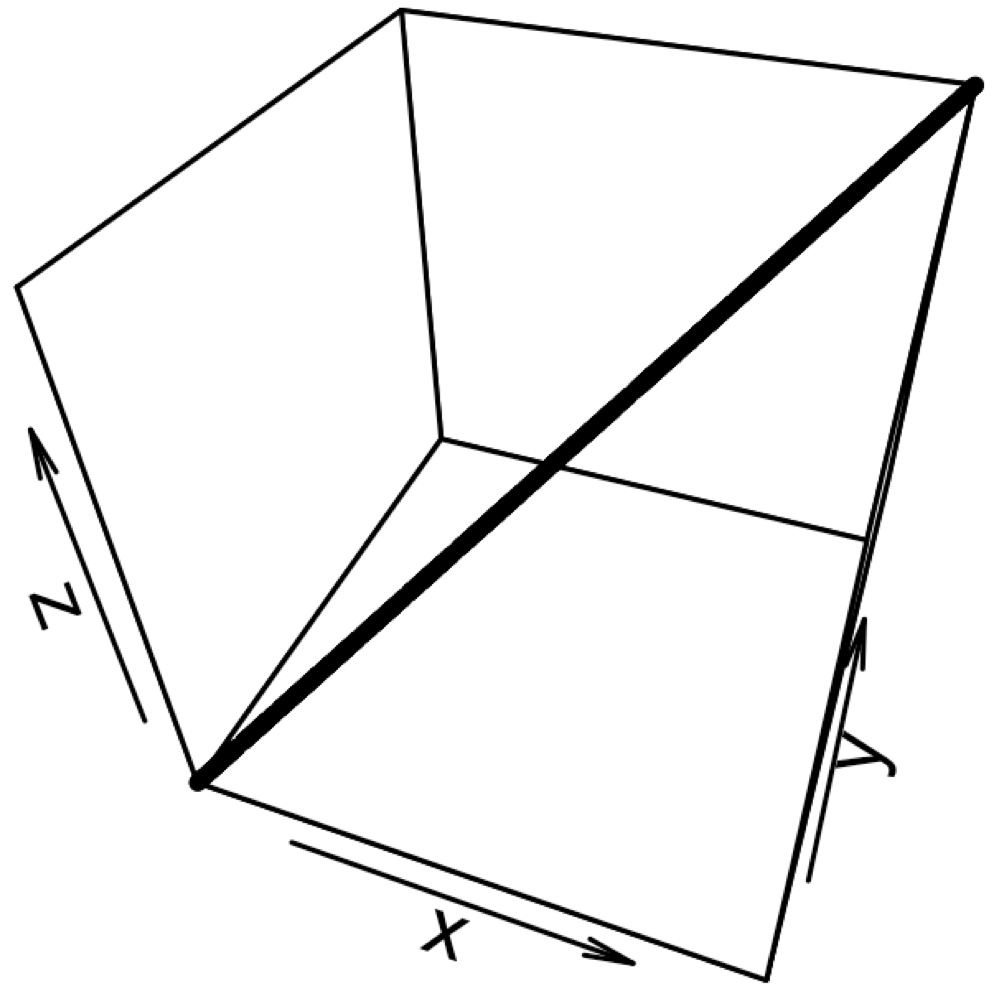
\includegraphics[width=.8\linewidth]{Ej5_scuniforme.png}  
  \caption{3D of function \texttt{uniforme}(2000, 27)}
  \label{extra3}
\end{subfigure}
\caption{3D depiction of each uniform random number generator}
\label{extra}
\end{figure}


\section{Conclusions}

It was really interesting learning more about random numbers, since we use them so much when doing experimentations. It was also compelling seeing the difference between using a good seed and a bad one in the generation of uniform numbers, because in the first figures when we prove their uniformity there was no big sign that the results in the Gaussian experiment where going to behave that way. \\

There was also the expectation that in the experiments of changing the independent variables into dependent ones, that the histograms would look a lot more weird than the ones with independent variables, if only because in class there was the idea that taking away the independence of the variables would ruin the outcome of the Gaussian experiment.\\
\bibliographystyle{plainnat}
\bibliography{tarea5}


 
\end{document}